\subsection{Method Overview}

This section details our method for achieving the goals laid out in Section \ref{objectives}. The objective is to identify map points which, while previously viewed, are no longer visible due to environmental changes. To address this, we assign an incrementally updated probability of existence value to each map point. Observations of a map point increase our overall confidence in its existence. Conversely, failure to observe a map point from a viewpoint where it \textit{should} have been visible lowers our confidence in its existence. Determining whether a map point should be observable from a given viewpoint is not trivial, motivating the need for a viewpoint-aware observability model. The purpose of the model is to integrate historical observability data to estimate observability across all possible viewpoints.

\subsubsection{The Bayesian Update Step}

The system updates its confidence for a map point's existence based on environmental observations. This update follows Bayes' theorem, and can therefore be implemented to utilize Bayesian statistics. The events of interest are:
\begin{itemize}
    \item $E$: The event that the map point exists
    \item $S^{\boldsymbol{v}}$: The event that the map point is seen from viewpoint $\boldsymbol{v}$
\end{itemize}

where $\boldsymbol{v} = \{\theta,\phi,d\}$, representing azimuth, elevation and distance from the observer to the point respectively. To formalize, our system updates $P(E) = P(E|S^{\boldsymbol{v}})$ given a positive observation, and $P(E) = P(E|\neg S^{\boldsymbol{v}})$ given a negative observation.

Applying Bayes' theorem, the derived update function is
\[
    P(E) = \begin{cases}
        \frac{P(S^{\boldsymbol{v}}|E)P(E)}{P(S^{\boldsymbol{v}})}           & \text{given }S^{\boldsymbol{v}}      \\
        \frac{P(\neg S^{\boldsymbol{v}}|E)P(E)}{P(\neg S^{\boldsymbol{v}})} & \text{given }\neg S^{\boldsymbol{v}}
    \end{cases}
\]

Additionally, the marginal probability $P(S^{\boldsymbol{v}})$ is
$$
    P(S^{\boldsymbol{v}}) = P(S^{\boldsymbol{v}}|E)P(E) + P(S^{\boldsymbol{v}}|\neg E)P(\neg E)
$$

The probability of a false observation of of a non-existent map point is small, but non-zero. The probability of a false match increases in low-light and in low texture environments. The value $\varepsilon$ is assigned to represent this probability, and will be experimentally determined in Section \ref{sec:existence_confidence_eval}.
$$
    \varepsilon = P(S^{\boldsymbol{v}}|\neg E) \approx 0
$$

Finally, assuming the existence of a model function $m$ which estimates the probability of observing the point from a given viewpoint $\boldsymbol{v}$
$$
    m(\boldsymbol{v}) \approx P(S^{\boldsymbol{v}}|E)
$$

The update step can be expressed as
\[
    P(E) = \begin{cases}
        \frac{m(\boldsymbol{v})P(E)}{m(\boldsymbol{v})P(E) + \varepsilon(1-P(E))}             & \text{given }S^{\boldsymbol{v}}      \\
        \frac{(1-m(\boldsymbol{v}))P(E)}{(1-m(\boldsymbol{v}))P(E) + (1-\varepsilon)(1-P(E))} & \text{given }\neg S^{\boldsymbol{v}}
    \end{cases}
\]

\subsubsection{The Observability of Map Points}

For the purposes of KV-SLAM, map features can be conceptualized as static, infinitesimally small points in 3D space. Because they have no width or height, a map feature can never be partially obscured, and are immune to perspective. This means that the visibility of a map feature can be represented by the function
$$
    v:(\theta,\phi,d):[0,2\pi)\times\left[-\frac{\pi}{2},\frac{\pi}{2}\right]\times[0,\infty)\to{0,1}
$$
where $\theta\in[0,2\pi)$ represents the azimuth, $\phi\in\left[-\frac{\pi}{2},\frac{\pi}{2}\right]$ represents the elevation, and $d\in[0,\infty)$ represents the distance between the map feature and the observer. This visibility function returns 1 if the point is observable from the input viewpoint, and 0 if it is not. From this, observations can be defined as $o=\{\theta,\phi,v(\theta,\phi)\}\in[0,2\pi)\times\left[-\frac{\pi}{2},\frac{\pi}{2}\right]\times\{0,1\}$ For illustrative purposes, The left plot of Figure \ref{fig:2d_observability} represents the output of a simplified 2D version of the observability function across the domain of $\theta\times d$, and the effects of obstructions on the observability. However, to generate such a plot from sensor data would require infinite observations spanning the full domain of $\theta\times d$. Instead, the system must operate on a finite set of observations as shown in the plot on the right. As described above, the Bayesian update step requires a model function $m$,
\begin{figure}[!ht]
    \centering
    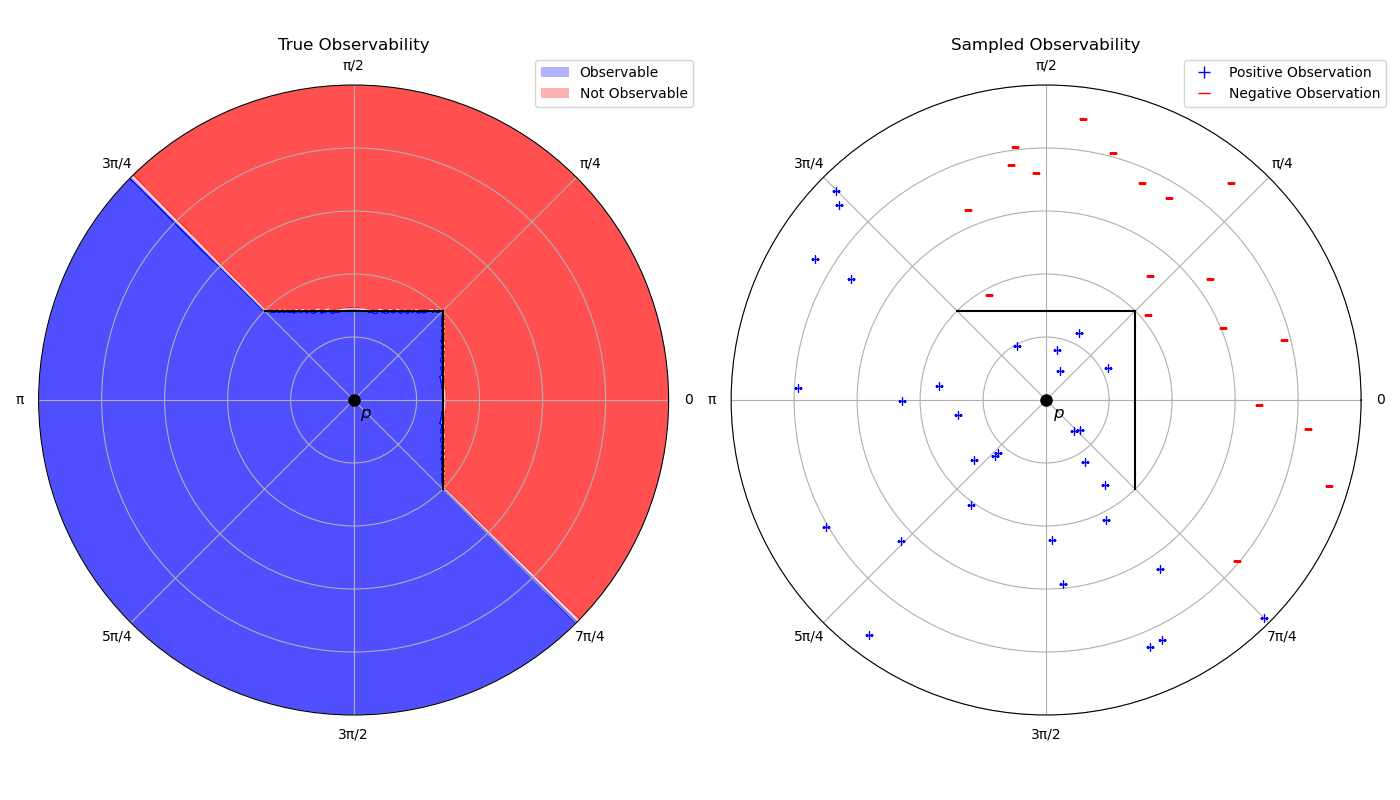
\includegraphics[width=0.9\textwidth]{resources/2d_observability.png}
    \caption[2D Observability]{(Left) A 2D representation of the true observability of a map point when near two orthogonal obstructions. (Right) A 2D representation of 100 observations of a map point near two orthogonal obstructions.}
    \label{fig:2d_observability}
\end{figure}

\subsubsection{Modeling Historical Observability of Map Points}

The goal of the model is to estimate the global observability of a point using a finite set of $n$ observations $\boldsymbol{O} = \{o_0,\dots,o_n\}$, and a current viewpoint $v=\{\theta,\phi,d\}$. Observations take the form $o_n=\{\theta_n,\phi_n,d_n,seen_n\}$, so the model can be written
$$
    m(\boldsymbol{O},\theta,\phi,d)\to[0,1]
$$

Therefore, the model function will be selected with the goal of minimizing the objective function
$$
    \iiint |m(\boldsymbol{O},\theta,\phi,d) - v(\theta,\phi,d)| \,d\theta\,d\phi\,dd
$$

Three implementations of the model $m$ will be implemented, and will have their parameters optimized in simulation. Each will be tested on the datasets produced for this research. With perfect sampling,
